\documentclass[12pt,a4paper]{article}

\usepackage[a4paper,text={16.5cm,25.2cm},centering]{geometry}
\usepackage{lmodern}
\usepackage{amssymb,amsmath}
\usepackage{bm}
\usepackage{graphicx}
\usepackage{microtype}
\usepackage{hyperref}
\setlength{\parindent}{0pt}
\setlength{\parskip}{1.2ex}

\hypersetup
       {   pdfauthor = { Marco Fasondini },
           pdftitle={ foo },
           colorlinks=TRUE,
           linkcolor=black,
           citecolor=blue,
           urlcolor=blue
       }




\usepackage{upquote}
\usepackage{listings}
\usepackage{xcolor}
\lstset{
    basicstyle=\ttfamily\footnotesize,
    upquote=true,
    breaklines=true,
    breakindent=0pt,
    keepspaces=true,
    showspaces=false,
    columns=fullflexible,
    showtabs=false,
    showstringspaces=false,
    escapeinside={(*@}{@*)},
    extendedchars=true,
}
\newcommand{\HLJLt}[1]{#1}
\newcommand{\HLJLw}[1]{#1}
\newcommand{\HLJLe}[1]{#1}
\newcommand{\HLJLeB}[1]{#1}
\newcommand{\HLJLo}[1]{#1}
\newcommand{\HLJLk}[1]{\textcolor[RGB]{148,91,176}{\textbf{#1}}}
\newcommand{\HLJLkc}[1]{\textcolor[RGB]{59,151,46}{\textit{#1}}}
\newcommand{\HLJLkd}[1]{\textcolor[RGB]{214,102,97}{\textit{#1}}}
\newcommand{\HLJLkn}[1]{\textcolor[RGB]{148,91,176}{\textbf{#1}}}
\newcommand{\HLJLkp}[1]{\textcolor[RGB]{148,91,176}{\textbf{#1}}}
\newcommand{\HLJLkr}[1]{\textcolor[RGB]{148,91,176}{\textbf{#1}}}
\newcommand{\HLJLkt}[1]{\textcolor[RGB]{148,91,176}{\textbf{#1}}}
\newcommand{\HLJLn}[1]{#1}
\newcommand{\HLJLna}[1]{#1}
\newcommand{\HLJLnb}[1]{#1}
\newcommand{\HLJLnbp}[1]{#1}
\newcommand{\HLJLnc}[1]{#1}
\newcommand{\HLJLncB}[1]{#1}
\newcommand{\HLJLnd}[1]{\textcolor[RGB]{214,102,97}{#1}}
\newcommand{\HLJLne}[1]{#1}
\newcommand{\HLJLneB}[1]{#1}
\newcommand{\HLJLnf}[1]{\textcolor[RGB]{66,102,213}{#1}}
\newcommand{\HLJLnfm}[1]{\textcolor[RGB]{66,102,213}{#1}}
\newcommand{\HLJLnp}[1]{#1}
\newcommand{\HLJLnl}[1]{#1}
\newcommand{\HLJLnn}[1]{#1}
\newcommand{\HLJLno}[1]{#1}
\newcommand{\HLJLnt}[1]{#1}
\newcommand{\HLJLnv}[1]{#1}
\newcommand{\HLJLnvc}[1]{#1}
\newcommand{\HLJLnvg}[1]{#1}
\newcommand{\HLJLnvi}[1]{#1}
\newcommand{\HLJLnvm}[1]{#1}
\newcommand{\HLJLl}[1]{#1}
\newcommand{\HLJLld}[1]{\textcolor[RGB]{148,91,176}{\textit{#1}}}
\newcommand{\HLJLs}[1]{\textcolor[RGB]{201,61,57}{#1}}
\newcommand{\HLJLsa}[1]{\textcolor[RGB]{201,61,57}{#1}}
\newcommand{\HLJLsb}[1]{\textcolor[RGB]{201,61,57}{#1}}
\newcommand{\HLJLsc}[1]{\textcolor[RGB]{201,61,57}{#1}}
\newcommand{\HLJLsd}[1]{\textcolor[RGB]{201,61,57}{#1}}
\newcommand{\HLJLsdB}[1]{\textcolor[RGB]{201,61,57}{#1}}
\newcommand{\HLJLsdC}[1]{\textcolor[RGB]{201,61,57}{#1}}
\newcommand{\HLJLse}[1]{\textcolor[RGB]{59,151,46}{#1}}
\newcommand{\HLJLsh}[1]{\textcolor[RGB]{201,61,57}{#1}}
\newcommand{\HLJLsi}[1]{#1}
\newcommand{\HLJLso}[1]{\textcolor[RGB]{201,61,57}{#1}}
\newcommand{\HLJLsr}[1]{\textcolor[RGB]{201,61,57}{#1}}
\newcommand{\HLJLss}[1]{\textcolor[RGB]{201,61,57}{#1}}
\newcommand{\HLJLssB}[1]{\textcolor[RGB]{201,61,57}{#1}}
\newcommand{\HLJLnB}[1]{\textcolor[RGB]{59,151,46}{#1}}
\newcommand{\HLJLnbB}[1]{\textcolor[RGB]{59,151,46}{#1}}
\newcommand{\HLJLnfB}[1]{\textcolor[RGB]{59,151,46}{#1}}
\newcommand{\HLJLnh}[1]{\textcolor[RGB]{59,151,46}{#1}}
\newcommand{\HLJLni}[1]{\textcolor[RGB]{59,151,46}{#1}}
\newcommand{\HLJLnil}[1]{\textcolor[RGB]{59,151,46}{#1}}
\newcommand{\HLJLnoB}[1]{\textcolor[RGB]{59,151,46}{#1}}
\newcommand{\HLJLoB}[1]{\textcolor[RGB]{102,102,102}{\textbf{#1}}}
\newcommand{\HLJLow}[1]{\textcolor[RGB]{102,102,102}{\textbf{#1}}}
\newcommand{\HLJLp}[1]{#1}
\newcommand{\HLJLc}[1]{\textcolor[RGB]{153,153,119}{\textit{#1}}}
\newcommand{\HLJLch}[1]{\textcolor[RGB]{153,153,119}{\textit{#1}}}
\newcommand{\HLJLcm}[1]{\textcolor[RGB]{153,153,119}{\textit{#1}}}
\newcommand{\HLJLcp}[1]{\textcolor[RGB]{153,153,119}{\textit{#1}}}
\newcommand{\HLJLcpB}[1]{\textcolor[RGB]{153,153,119}{\textit{#1}}}
\newcommand{\HLJLcs}[1]{\textcolor[RGB]{153,153,119}{\textit{#1}}}
\newcommand{\HLJLcsB}[1]{\textcolor[RGB]{153,153,119}{\textit{#1}}}
\newcommand{\HLJLg}[1]{#1}
\newcommand{\HLJLgd}[1]{#1}
\newcommand{\HLJLge}[1]{#1}
\newcommand{\HLJLgeB}[1]{#1}
\newcommand{\HLJLgh}[1]{#1}
\newcommand{\HLJLgi}[1]{#1}
\newcommand{\HLJLgo}[1]{#1}
\newcommand{\HLJLgp}[1]{#1}
\newcommand{\HLJLgs}[1]{#1}
\newcommand{\HLJLgsB}[1]{#1}
\newcommand{\HLJLgt}[1]{#1}



\def\qqand{\qquad\hbox{and}\qquad}
\def\qqfor{\qquad\hbox{for}\qquad}
\def\qqas{\qquad\hbox{as}\qquad}
\def\half{ {1 \over 2} }
\def\D{ {\rm d} }
\def\I{ {\rm i} }
\def\E{ {\rm e} }
\def\C{ {\mathbb C} }
\def\R{ {\mathbb R} }
\def\H{ {\mathbb H} }
\def\Z{ {\mathbb Z} }
\def\CC{ {\cal C} }
\def\FF{ {\cal F} }
\def\HH{ {\cal H} }
\def\LL{ {\cal L} }
\def\vc#1{ {\mathbf #1} }
\def\bbC{ {\mathbb C} }



\def\fR{ f_{\rm R} }
\def\fL{ f_{\rm L} }

\def\qqqquad{\qquad\qquad}
\def\qqwhere{\qquad\hbox{where}\qquad}
\def\Res_#1{\underset{#1}{\rm Res}\,}
\def\sech{ {\rm sech}\, }
\def\acos{ {\rm acos}\, }
\def\asin{ {\rm asin}\, }
\def\atan{ {\rm atan}\, }
\def\Ei{ {\rm Ei}\, }
\def\upepsilon{\varepsilon}


\def\Xint#1{ \mathchoice
   {\XXint\displaystyle\textstyle{#1} }%
   {\XXint\textstyle\scriptstyle{#1} }%
   {\XXint\scriptstyle\scriptscriptstyle{#1} }%
   {\XXint\scriptscriptstyle\scriptscriptstyle{#1} }%
   \!\int}
\def\XXint#1#2#3{ {\setbox0=\hbox{$#1{#2#3}{\int}$}
     \vcenter{\hbox{$#2#3$}}\kern-.5\wd0} }
\def\ddashint{\Xint=}
\def\dashint{\Xint-}
% \def\dashint
\def\infdashint{\dashint_{-\infty}^\infty}




\def\addtab#1={#1\;&=}
\def\ccr{\\\addtab}
\def\ip<#1>{\left\langle{#1}\right\rangle}
\def\dx{\D x}
\def\dt{\D t}
\def\dz{\D z}
\def\ds{\D s}

\def\rR{ {\rm R} }
\def\rL{ {\rm L} }

\def\norm#1{\left\| #1 \right\|}

\def\pr(#1){\left({#1}\right)}
\def\br[#1]{\left[{#1}\right]}

\def\abs#1{\left|{#1}\right|}
\def\fpr(#1){\!\pr({#1})}

\def\sopmatrix#1{ \begin{pmatrix}#1\end{pmatrix} }

\def\endash{–}
\def\emdash{—}
\def\mdblksquare{\blacksquare}
\def\lgblksquare{\blacksquare}
\def\scre{\E}
\def\mapengine#1,#2.{\mapfunction{#1}\ifx\void#2\else\mapengine #2.\fi }

\def\map[#1]{\mapengine #1,\void.}

\def\mapenginesep_#1#2,#3.{\mapfunction{#2}\ifx\void#3\else#1\mapengine #3.\fi }

\def\mapsep_#1[#2]{\mapenginesep_{#1}#2,\void.}


\def\vcbr[#1]{\pr(#1)}


\def\bvect[#1,#2]{
{
\def\dots{\cdots}
\def\mapfunction##1{\ | \  ##1}
	\sopmatrix{
		 \,#1\map[#2]\,
	}
}
}



\def\vect[#1]{
{\def\dots{\ldots}
	\vcbr[{#1}]
} }

\def\vectt[#1]{
{\def\dots{\ldots}
	\vect[{#1}]^{\top}
} }

\def\Vectt[#1]{
{
\def\mapfunction##1{##1 \cr}
\def\dots{\vdots}
	\begin{pmatrix}
		\map[#1]
	\end{pmatrix}
} }

\def\addtab#1={#1\;&=}
\def\ccr{\\\addtab}

\def\questionequals{= \!\!\!\!\!\!{\scriptstyle ? \atop }\,\,\,}

\begin{document}

\textbf{Applied Complex Analysis (2021)}

\section{Lecture 4: Analyticity at infinity}
In this lecture we cover

\begin{itemize}
\item[1. ] Riemann sphere and analyticity at infinity


\item[2. ] Cauchy's theorem and Cauchy's integral formula, exterior to a contour


\item[3. ] Exterior Residue theorem

\end{itemize}
\subsection{Riemann sphere and analyticity at infinity}
\textbf{Definition (Riemann sphere)} The \emph{Riemann sphere} is the compactification of ${\mathbb C}$:

\[
    \bar {\mathbb C} = {\mathbb C} \cup \{\infty\}
\]
Without delving on the details, we can define an open set $D \subset \bar{\mathbb C}$ on the Riemann sphere, where $\infty \in D$ implies that there exists an $R$ such that $\{ z : |z| > R\} \subset D$.

\textbf{Definition (Analytic at infinity)} A function $f(z)$ defined on an open set $D \subset \bar {\mathbb C}$ such that $\infty \in D$ is \emph{analytic at \ensuremath{\infty}} if $f(z^{-1})$ is analytic at zero.

\textbf{Proposition (Taylor series at infinity)} If $f$ is analytic at infinity, then there exists an $R$ such that for all $|z| > R$ we have

\[
f(z) = \sum_{k=-\infty}^0 f_k z^k
\]
The coefficients $f_k$ are defined by

\[
f_k = {1 \over 2 \pi \I} \oint_\gamma {f(z) \over z^{k+1}} \dz
\]
where $\gamma$ is any simple closed positively oriented contour outside of which $f$ is analytic.

\textbf{Theorem (Cauchy's theorem, exterior)} Suppose $f$ is analytic outside and on a positively oriented, simple, closed contour $\gamma$, and

\[
f(z) = o(z^{-1})
\]
as $z \rightarrow \infty$. Then we have

\[
\oint_\gamma f(z) \D z = 0.
\]
\textbf{Proof} Follows by deforming $\gamma$ to a large circle and using $ML$ theorem. \ensuremath{\blacksquare}

\textbf{Theorem (Cauchy's integral theorem, exterior)} Suppose $f$ is analytic outside and on a positively oriented, simple, closed contour $\gamma$, and

\[
f(\infty) = 0,
\]
that is, $f(z)$ decays as $z \rightarrow \infty$. Then we have

\[
f(z) = -{1 \over 2 \pi \I} \oint {f(\zeta) \over \zeta - z} \D \zeta
\]
\emph{Demonstration} $f(z) = \E^{1/z}$ is not analytic at zero, but is analytic at infinity because $f(1/z) = \E^z$ is analytic at zero. We therefore have a convergent "Taylor" series in inverse powers of $z$:

\[
\E^{1/z} = 1 + {1 \over z} + {1 \over 2 z^2} + {1 \over 3! z^3} + \cdots
\]
Or seen numerically:


\begin{lstlisting}
(*@\HLJLn{z}@*) (*@\HLJLoB{=}@*) (*@\HLJLnfB{2.0}@*)(*@\HLJLoB{+}@*)(*@\HLJLni{2}@*)(*@\HLJLn{im}@*)
(*@\HLJLnf{sum}@*)(*@\HLJLp{([}@*)(*@\HLJLn{z}@*)(*@\HLJLoB{{\textasciicircum}}@*)(*@\HLJLn{k}@*)(*@\HLJLoB{/}@*)(*@\HLJLnf{factorial}@*)(*@\HLJLp{(}@*)(*@\HLJLoB{-}@*)(*@\HLJLnfB{1.0}@*)(*@\HLJLn{k}@*)(*@\HLJLp{)}@*) (*@\HLJLk{for}@*) (*@\HLJLn{k}@*)(*@\HLJLoB{=-}@*)(*@\HLJLni{100}@*)(*@\HLJLoB{:}@*)(*@\HLJLni{0}@*)(*@\HLJLp{])}@*) (*@\HLJLoB{-}@*) (*@\HLJLnf{exp}@*)(*@\HLJLp{(}@*)(*@\HLJLni{1}@*)(*@\HLJLoB{/}@*)(*@\HLJLn{z}@*)(*@\HLJLp{)}@*)
\end{lstlisting}

\begin{lstlisting}
2.220446049250313e-16 - 5.551115123125783e-17im
\end{lstlisting}


The function $f(z) = \E^{1/z} - 1$ vanishes at $\infty$ and so can thence be recovered as a Cauchy integral:


\begin{lstlisting}
(*@\HLJLk{using}@*) (*@\HLJLn{ApproxFun}@*)
(*@\HLJLn{f}@*) (*@\HLJLoB{=}@*) (*@\HLJLn{z}@*) (*@\HLJLoB{->}@*) (*@\HLJLnf{exp}@*)(*@\HLJLp{(}@*)(*@\HLJLni{1}@*)(*@\HLJLoB{/}@*)(*@\HLJLn{z}@*)(*@\HLJLp{)}@*) (*@\HLJLoB{-}@*) (*@\HLJLni{1}@*)

(*@\HLJLn{\ensuremath{\zeta}}@*) (*@\HLJLoB{=}@*) (*@\HLJLnf{Fun}@*)(*@\HLJLp{(}@*)(*@\HLJLnf{Circle}@*)(*@\HLJLp{())}@*)
(*@\HLJLoB{-}@*)(*@\HLJLnf{sum}@*)(*@\HLJLp{(}@*)(*@\HLJLn{f}@*)(*@\HLJLoB{.}@*)(*@\HLJLp{(}@*)(*@\HLJLn{\ensuremath{\zeta}}@*)(*@\HLJLp{)}@*)(*@\HLJLoB{/}@*)(*@\HLJLp{(}@*)(*@\HLJLn{\ensuremath{\zeta}}@*)(*@\HLJLoB{-}@*)(*@\HLJLn{z}@*)(*@\HLJLp{))}@*)(*@\HLJLoB{/}@*)(*@\HLJLp{(}@*)(*@\HLJLni{2}@*)(*@\HLJLn{\ensuremath{\pi}}@*)(*@\HLJLoB{*}@*)(*@\HLJLn{im}@*)(*@\HLJLp{)}@*) (*@\HLJLoB{-}@*) (*@\HLJLnf{f}@*)(*@\HLJLp{(}@*)(*@\HLJLn{z}@*)(*@\HLJLp{)}@*) (*@\HLJLcs{{\#}}@*) (*@\HLJLcs{compare}@*) (*@\HLJLcs{numerical}@*) (*@\HLJLcs{integral}@*) (*@\HLJLcs{with}@*) (*@\HLJLcs{{\textasciigrave}f{\textasciigrave}}@*)
\end{lstlisting}

\begin{lstlisting}
1.6653345369377348e-16 + 1.1102230246251565e-16im
\end{lstlisting}


The decay at infinity is required: for a function that does not decay, Cauchy's integral formula in the exterior fails:


\begin{lstlisting}
(*@\HLJLn{f}@*) (*@\HLJLoB{=}@*) (*@\HLJLn{z}@*) (*@\HLJLoB{->}@*) (*@\HLJLnf{exp}@*)(*@\HLJLp{(}@*)(*@\HLJLni{1}@*)(*@\HLJLoB{/}@*)(*@\HLJLn{z}@*)(*@\HLJLp{)}@*)

(*@\HLJLn{\ensuremath{\zeta}}@*) (*@\HLJLoB{=}@*) (*@\HLJLnf{Fun}@*)(*@\HLJLp{(}@*)(*@\HLJLnf{Circle}@*)(*@\HLJLp{())}@*)
(*@\HLJLoB{-}@*)(*@\HLJLnf{sum}@*)(*@\HLJLp{(}@*)(*@\HLJLn{f}@*)(*@\HLJLoB{.}@*)(*@\HLJLp{(}@*)(*@\HLJLn{\ensuremath{\zeta}}@*)(*@\HLJLp{)}@*)(*@\HLJLoB{/}@*)(*@\HLJLp{(}@*)(*@\HLJLn{\ensuremath{\zeta}}@*)(*@\HLJLoB{-}@*)(*@\HLJLn{z}@*)(*@\HLJLp{))}@*)(*@\HLJLoB{/}@*)(*@\HLJLp{(}@*)(*@\HLJLni{2}@*)(*@\HLJLn{\ensuremath{\pi}}@*)(*@\HLJLoB{*}@*)(*@\HLJLn{im}@*)(*@\HLJLp{)}@*) (*@\HLJLoB{-}@*) (*@\HLJLnf{f}@*)(*@\HLJLp{(}@*)(*@\HLJLn{z}@*)(*@\HLJLp{)}@*)
\end{lstlisting}

\begin{lstlisting}
-0.9999999999999998 + 1.6653345369377348e-16im
\end{lstlisting}


An alternative way of stating Cauchy's integral formula in the exterior is to add in the constant term: for any $f$ analytic at $\infty$ we have


\begin{align*}
f(z) &= -{1 \over 2 \pi \I} \oint_\gamma {f(\zeta) \over \zeta - z} \D \zeta  + f(\infty)  \\
    &= -{1 \over 2 \pi \I} \oint_\gamma {f(\zeta) \over \zeta - z} \D \zeta  + {1 \over 2 \pi \I} \oint_\gamma {f(z) \over z} \D z.
\end{align*}
\subsubsection{Exterior Residue theorem}
An analogue of residue calculus holds true counting over residues outside a contour, but we need to also include the residue at $\infty$.

\textbf{Definition (Residue at infinity)}  Suppose $f$ is analytic in the annulus $A_{R\infty} = \{z : R < |z| < \infty \}$. Then

\[
{\underset{z = \infty}{\rm Res}} \, f(z) = -f_{-1}
\]
where $f_{-1}$ is (again) the Laurent coefficient integrating over any circle $C_r$ in $A_{R\infty}$, that is $R < r < \infty$.

\textbf{Theorem (Exterior Residue Theorem)} Let $f$ be holomorphic outside and on a simple closed, positively oriented contour $\gamma$ except at isolated points $z_1, \ldots, z_r$ outside $\gamma$. Then

\[
\oint_\gamma f(z) \dz = -2 \pi \I \sum_{j=1}^r {\underset{z = z_j}{\rm Res}}\, f(z) - 2 \pi \I \Res_{z = \infty} f(z)
\]
\subsubsection{Examples}
Let's revisit the examples from before:


\begin{lstlisting}
(*@\HLJLk{using}@*) (*@\HLJLn{ApproxFun}@*)(*@\HLJLp{,}@*) (*@\HLJLn{Plots}@*)(*@\HLJLp{,}@*) (*@\HLJLn{ComplexPhasePortrait}@*)
(*@\HLJLn{f}@*) (*@\HLJLoB{=}@*) (*@\HLJLn{z}@*) (*@\HLJLoB{->}@*) (*@\HLJLni{1}@*)(*@\HLJLoB{/}@*)(*@\HLJLp{(}@*)(*@\HLJLn{z}@*)(*@\HLJLoB{*}@*)(*@\HLJLp{(}@*)(*@\HLJLn{z}@*)(*@\HLJLoB{+}@*)(*@\HLJLni{2}@*)(*@\HLJLp{))}@*)
(*@\HLJLnf{phaseplot}@*)(*@\HLJLp{(}@*)(*@\HLJLoB{-}@*)(*@\HLJLnfB{3..3}@*)(*@\HLJLp{,}@*) (*@\HLJLoB{-}@*)(*@\HLJLnfB{3..3}@*)(*@\HLJLp{,}@*) (*@\HLJLn{f}@*)(*@\HLJLp{)}@*)
\end{lstlisting}

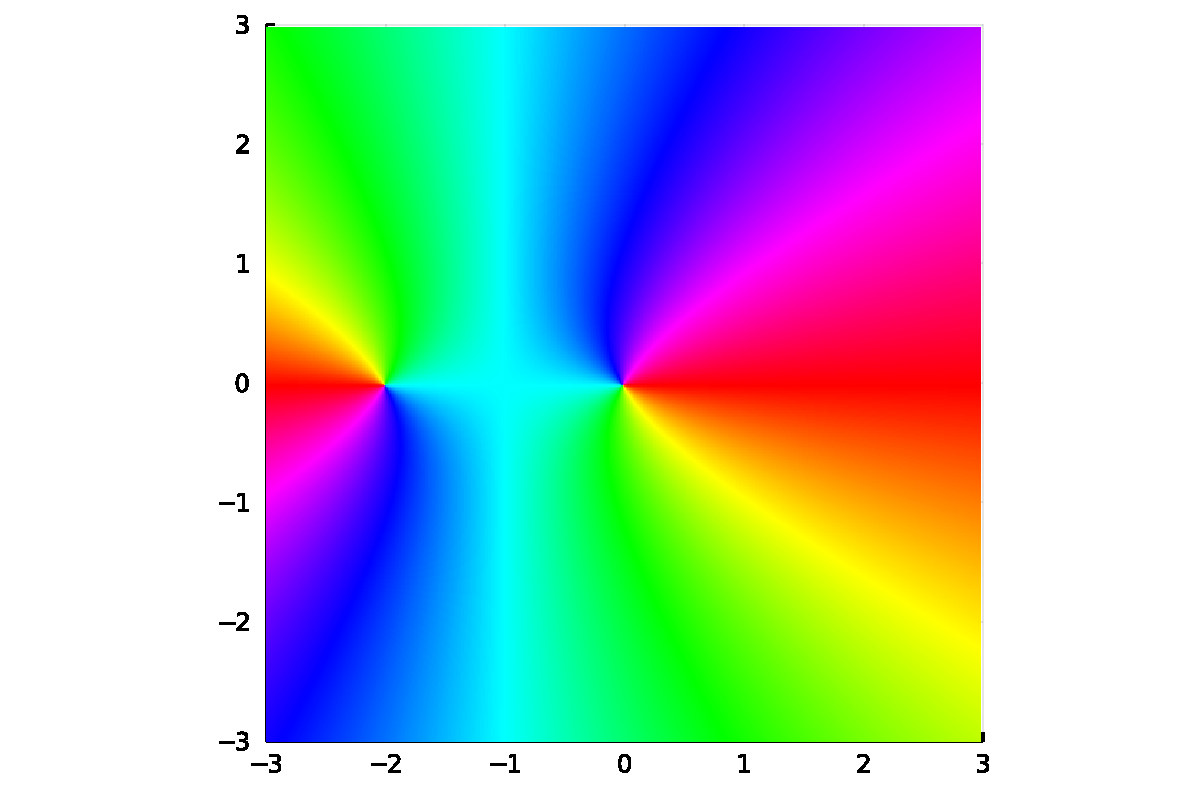
\includegraphics[width=\linewidth]{C:/Users/mfaso/OneDrive/Documents/GitHub/M3M6AppliedComplexAnalysis/output/figures/Lecture4_4_1.pdf}

Because it is analytic outside a circle of radius 3 and decays like $O(z^{-2})$, its residue at infinity is zero. Or in other words using the exterior version of Cauchy's integral formula. We can verify numerically:


\begin{lstlisting}
(*@\HLJLnf{sum}@*)(*@\HLJLp{(}@*)(*@\HLJLnf{Fun}@*)(*@\HLJLp{(}@*)(*@\HLJLn{f}@*)(*@\HLJLp{,}@*) (*@\HLJLnf{Circle}@*)(*@\HLJLp{(}@*)(*@\HLJLnfB{3.0}@*)(*@\HLJLp{)))}@*)
\end{lstlisting}

\begin{lstlisting}
2.362499203067714e-18 - 9.43464870604594e-17im
\end{lstlisting}


Here's another example with singularities at $0$ and $-2$:


\begin{lstlisting}
(*@\HLJLn{f}@*) (*@\HLJLoB{=}@*) (*@\HLJLn{z}@*) (*@\HLJLoB{->}@*) (*@\HLJLni{1}@*)(*@\HLJLoB{/}@*)(*@\HLJLn{z}@*) (*@\HLJLoB{+}@*) (*@\HLJLni{1}@*)(*@\HLJLoB{/}@*)(*@\HLJLp{(}@*)(*@\HLJLn{z}@*)(*@\HLJLoB{+}@*)(*@\HLJLni{2}@*)(*@\HLJLp{)}@*)
(*@\HLJLnf{phaseplot}@*)(*@\HLJLp{(}@*)(*@\HLJLoB{-}@*)(*@\HLJLnfB{3..3}@*)(*@\HLJLp{,}@*) (*@\HLJLoB{-}@*)(*@\HLJLnfB{3..3}@*)(*@\HLJLp{,}@*) (*@\HLJLn{f}@*)(*@\HLJLp{)}@*)
\end{lstlisting}

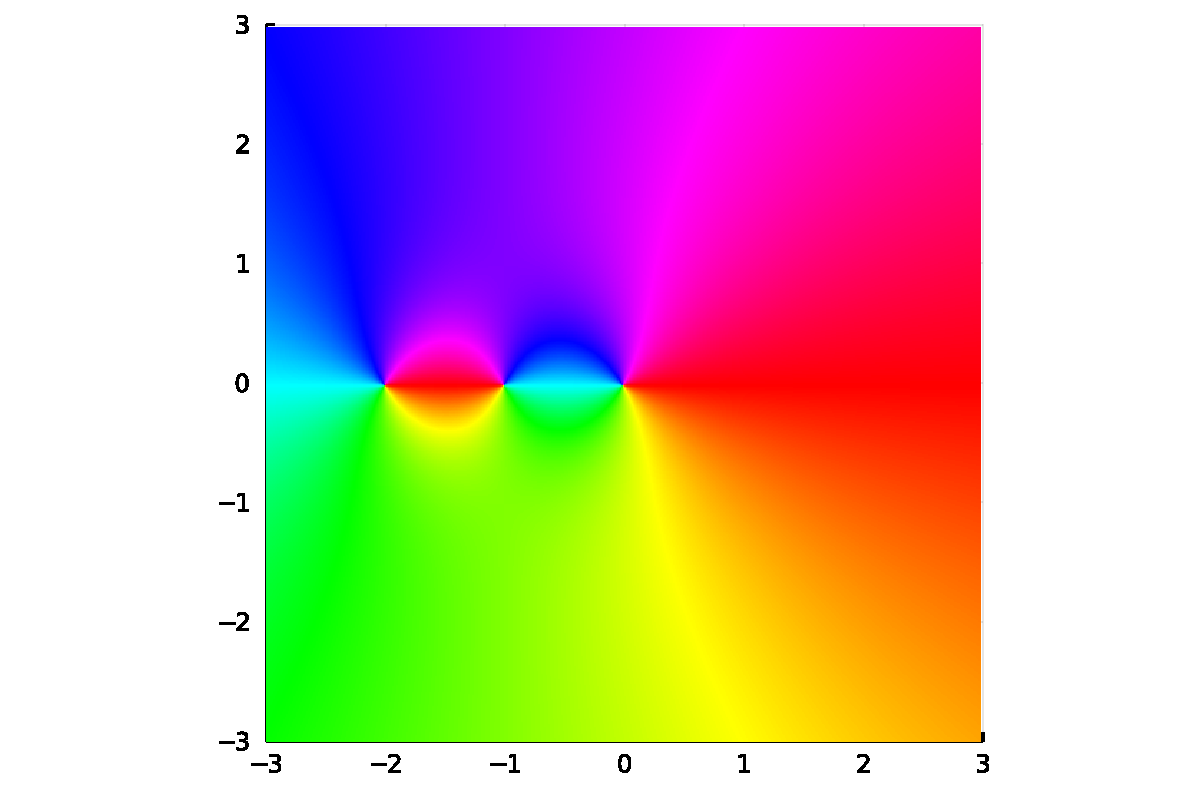
\includegraphics[width=\linewidth]{C:/Users/mfaso/OneDrive/Documents/GitHub/M3M6AppliedComplexAnalysis/output/figures/Lecture4_6_1.pdf}

This has a residue at infinity:

\[
f(z) = {2 \over z} + O(z^{-2})
\]
implies

\[
\Res_{z = \infty} f(z) = -2
\]
Thus an integral over a circle of radius 3 equals

\[
\oint_{C_3} f \D z = -2 \pi \I \Res_{z = \infty} f = 4\pi \I
\]
which matches the interior residue calculus

\[
\oint_{C_3} f \D z =  2 \pi \I \pr(\Res_{z = 0} + \Res_{z = -2}) f = 4 \pi \I
\]
If we had a circle of radius 1 then the exterior computation has two contributions:

\[
\oint_{C_1} f \D z =  -2 \pi \I \pr(\Res_{z = -2} + \Res_{z = \infty}) f = 2\pi \I
\]
which matches the interior residue calculation.


\begin{lstlisting}
(*@\HLJLnf{sum}@*)(*@\HLJLp{(}@*)(*@\HLJLnf{Fun}@*)(*@\HLJLp{(}@*)(*@\HLJLn{f}@*)(*@\HLJLp{,}@*) (*@\HLJLnf{Circle}@*)(*@\HLJLp{(}@*)(*@\HLJLnfB{3.0}@*)(*@\HLJLp{)))}@*)(*@\HLJLoB{-}@*)(*@\HLJLni{4}@*)(*@\HLJLn{\ensuremath{\pi}}@*)(*@\HLJLoB{*}@*)(*@\HLJLn{im}@*)(*@\HLJLp{,}@*) (*@\HLJLnf{sum}@*)(*@\HLJLp{(}@*)(*@\HLJLnf{Fun}@*)(*@\HLJLp{(}@*)(*@\HLJLn{f}@*)(*@\HLJLp{,}@*) (*@\HLJLnf{Circle}@*)(*@\HLJLp{(}@*)(*@\HLJLnfB{1.0}@*)(*@\HLJLp{)))}@*)(*@\HLJLoB{-}@*)(*@\HLJLni{2}@*)(*@\HLJLn{\ensuremath{\pi}}@*)(*@\HLJLoB{*}@*)(*@\HLJLn{im}@*)
\end{lstlisting}

\begin{lstlisting}
(-1.7090812387796532e-15 + 1.7763568394002505e-15im, -9.522127519313684e-16
 + 0.0im)
\end{lstlisting}


An example with singularities that are not isolated:


\begin{lstlisting}
(*@\HLJLn{f}@*) (*@\HLJLoB{=}@*) (*@\HLJLn{z}@*) (*@\HLJLoB{->}@*) (*@\HLJLnf{sqrt}@*)(*@\HLJLp{(}@*)(*@\HLJLn{z}@*)(*@\HLJLoB{-}@*)(*@\HLJLni{1}@*)(*@\HLJLp{)}@*)(*@\HLJLoB{*}@*)(*@\HLJLnf{sqrt}@*)(*@\HLJLp{(}@*)(*@\HLJLn{z}@*)(*@\HLJLoB{+}@*)(*@\HLJLni{1}@*)(*@\HLJLp{)}@*)(*@\HLJLoB{/}@*)(*@\HLJLp{(}@*)(*@\HLJLn{z}@*)(*@\HLJLoB{{\textasciicircum}}@*)(*@\HLJLni{2}@*)(*@\HLJLoB{+}@*)(*@\HLJLni{4}@*)(*@\HLJLp{)}@*)
(*@\HLJLnf{phaseplot}@*)(*@\HLJLp{(}@*)(*@\HLJLoB{-}@*)(*@\HLJLnfB{3..3}@*)(*@\HLJLp{,}@*) (*@\HLJLoB{-}@*)(*@\HLJLnfB{3..3}@*)(*@\HLJLp{,}@*) (*@\HLJLn{f}@*)(*@\HLJLp{)}@*)
\end{lstlisting}

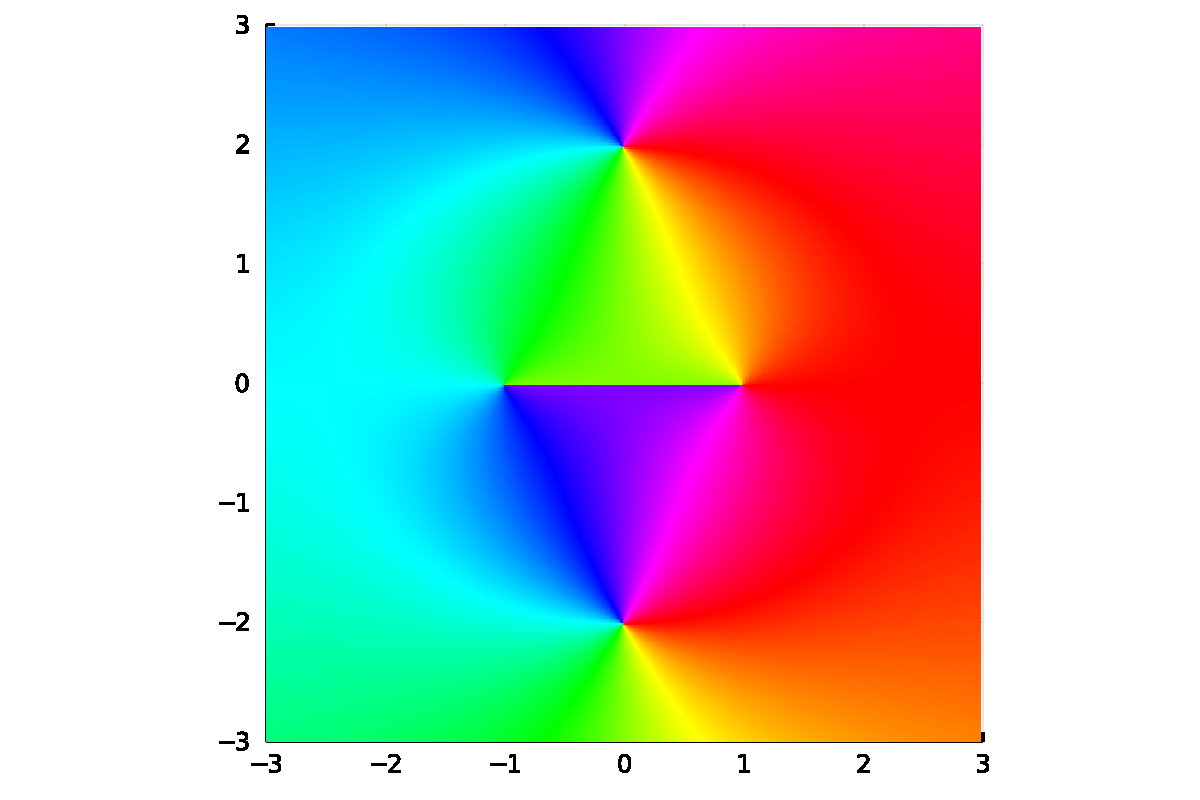
\includegraphics[width=\linewidth]{C:/Users/mfaso/OneDrive/Documents/GitHub/M3M6AppliedComplexAnalysis/output/figures/Lecture4_8_1.pdf}

The integral over the positively oriented circle of radius $r$ centred at the origin is

\[
\oint_{C_r} f \D z = 2 \pi \I \pr(\Res_{z = 2\I} f +  \Res_{z = -2\I} f +  \Res_{C_{\rho}} f) = -2 \pi \I \Res_{z = \infty} f,
\]
where $1 < \rho < 2$. Calculating the residue on $C_{\rho}$ is difficult but finding the residue at $z = \infty$ is much easier: for $z \rightarrow \infty$,

\[
f(z) = {1 \over z} + O(z^{-2}),
\]
hence

\[
\oint_{C_r} f \D z = -2 \pi \I \Res_{z = \infty} f = 2\pi \I.
\]

\begin{lstlisting}
(*@\HLJLnf{sum}@*)(*@\HLJLp{(}@*)(*@\HLJLnf{Fun}@*)(*@\HLJLp{(}@*)(*@\HLJLn{f}@*)(*@\HLJLp{,}@*) (*@\HLJLnf{Circle}@*)(*@\HLJLp{(}@*)(*@\HLJLnfB{3.0}@*)(*@\HLJLp{)))}@*)(*@\HLJLoB{/}@*)(*@\HLJLp{(}@*)(*@\HLJLni{2}@*)(*@\HLJLn{\ensuremath{\pi}}@*)(*@\HLJLoB{*}@*)(*@\HLJLn{im}@*)(*@\HLJLp{)}@*)
\end{lstlisting}

\begin{lstlisting}
1.0000000000000002 + 9.111995372164934e-17im
\end{lstlisting}


Here's a more complicated example:


\begin{lstlisting}
(*@\HLJLn{f}@*) (*@\HLJLoB{=}@*) (*@\HLJLn{z}@*) (*@\HLJLoB{->}@*) (*@\HLJLp{(}@*)(*@\HLJLn{z}@*)(*@\HLJLoB{+}@*)(*@\HLJLni{1}@*)(*@\HLJLp{)}@*)(*@\HLJLoB{*}@*)(*@\HLJLnf{exp}@*)(*@\HLJLp{(}@*)(*@\HLJLni{1}@*)(*@\HLJLoB{/}@*)(*@\HLJLn{z}@*)(*@\HLJLp{)}@*)(*@\HLJLoB{/}@*)(*@\HLJLp{(}@*)(*@\HLJLn{z}@*)(*@\HLJLoB{*}@*)(*@\HLJLp{(}@*)(*@\HLJLn{z}@*)(*@\HLJLoB{+}@*)(*@\HLJLni{2}@*)(*@\HLJLp{))}@*)
(*@\HLJLnf{phaseplot}@*)(*@\HLJLp{(}@*)(*@\HLJLoB{-}@*)(*@\HLJLnfB{3..3}@*)(*@\HLJLp{,}@*) (*@\HLJLoB{-}@*)(*@\HLJLnfB{3..3}@*)(*@\HLJLp{,}@*) (*@\HLJLn{f}@*)(*@\HLJLp{)}@*)
\end{lstlisting}

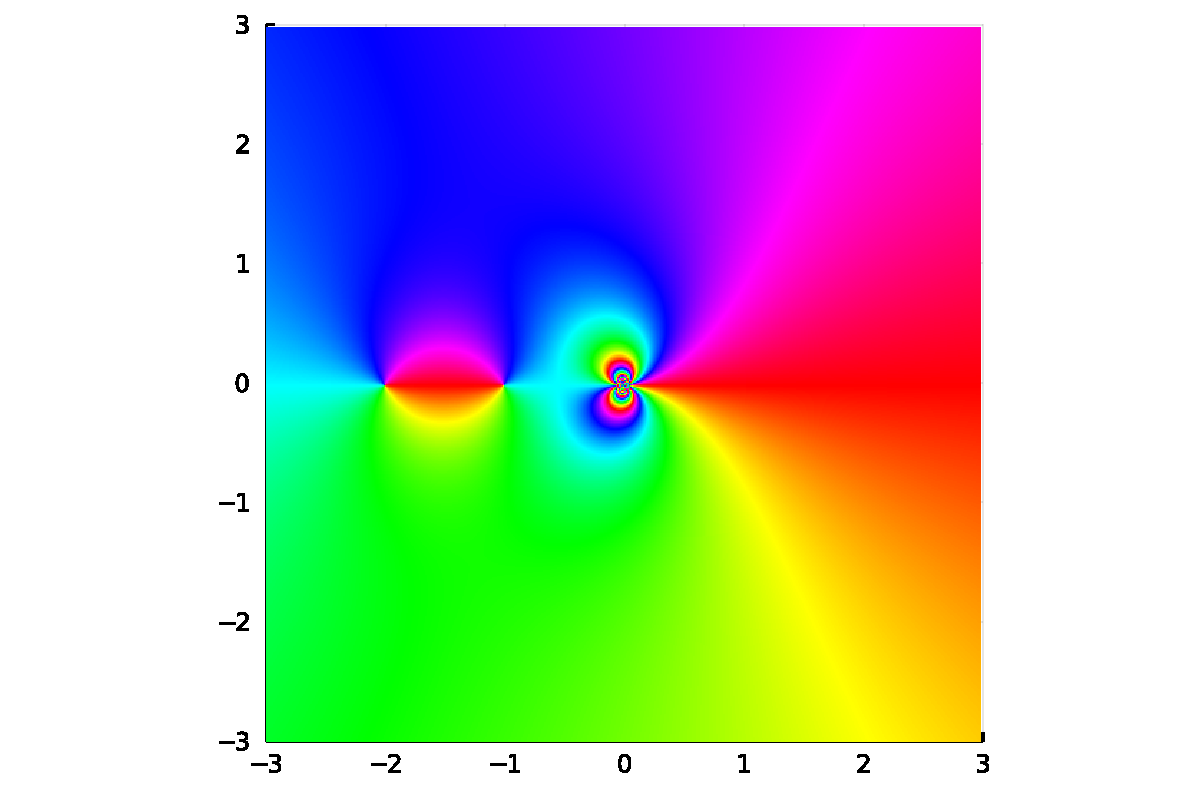
\includegraphics[width=\linewidth]{C:/Users/mfaso/OneDrive/Documents/GitHub/M3M6AppliedComplexAnalysis/output/figures/Lecture4_10_1.pdf}

This example has an essential singularity at zero so the classical Residue theorem is not much use, but we can use the residue theorem at infinity with the Laurent series (valid for large $z$)

\[
f(z) = 1/z + O(z^{-3})
\]
to determine

\[
\oint_{C_1} f \D z = - 2\pi \I \pr(\Res_{z=-2} + \Res_{z = \infty}) f(z) = -2 \pi \I ({1 \over 2 \E^{1/2}} - 1).
\]

\begin{lstlisting}
(*@\HLJLnf{sum}@*)(*@\HLJLp{(}@*)(*@\HLJLnf{Fun}@*)(*@\HLJLp{(}@*)(*@\HLJLn{f}@*)(*@\HLJLp{,}@*) (*@\HLJLnf{Circle}@*)(*@\HLJLp{(}@*)(*@\HLJLnfB{1.0}@*)(*@\HLJLp{)))}@*) (*@\HLJLoB{+}@*) (*@\HLJLni{2}@*)(*@\HLJLn{\ensuremath{\pi}}@*)(*@\HLJLoB{*}@*)(*@\HLJLn{im}@*)(*@\HLJLoB{*}@*)(*@\HLJLp{(}@*)(*@\HLJLnfB{0.5}@*)(*@\HLJLoB{*}@*)(*@\HLJLnf{exp}@*)(*@\HLJLp{(}@*)(*@\HLJLoB{-}@*)(*@\HLJLnfB{0.5}@*)(*@\HLJLp{)}@*)(*@\HLJLoB{-}@*)(*@\HLJLni{1}@*)(*@\HLJLp{)}@*)
\end{lstlisting}

\begin{lstlisting}
-6.259793792554635e-16 - 8.881784197001252e-16im
\end{lstlisting}



\end{document}
